\documentclass[10pt]{standalone}
\usepackage[sc]{mathpazo}
\usepackage{commands}

\begin{document}
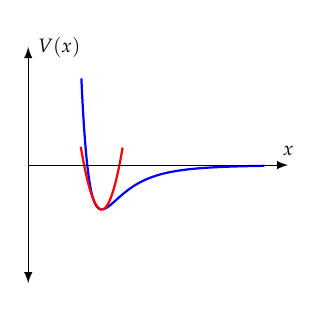
\begin{tikzpicture}[scale=1.5]
    \draw[scale=1, domain=0.95:2.5, smooth, samples=200, variable=\x, blue, thick]  plot ({\x}, {1.5*((1/(\x))^(12) - (1/(\x)^6))});
    \draw[scale=1, domain=0.945:1.3, smooth, samples=200, variable=\x, red, thick] plot ({(\x)}, {(4.1*(\x - 1.1225))^2-0.375});
    \draw[latex-latex] (0.5, -1) -- (0.5, 1);
    \draw[-latex] (0.5, 0) -- (2.7, 0);
    \node[above] at (2.7, 0) {\scriptsize $x$};
    \node[right] at (0.5, 1) {\scriptsize $V(x)$};
\end{tikzpicture}
\end{document}